\subsection{Discovering the Wonders of Zepp Antennas!}

\begin{tcolorbox}[colback=gray!10, colframe=black, title=E9C10] Which of the following describes a Zepp antenna? 
\begin{enumerate}[label=\Alph*.]
    \item A horizontal array capable of quickly changing the direction of maximum radiation by changing phasing lines
    \item \textbf{An end-fed half-wavelength dipole}
    \item An omni-directional antenna commonly used for satellite communications
    \item A vertical array capable of quickly changing the direction of maximum radiation by changing phasing lines
\end{enumerate} \end{tcolorbox}

A Zepp antenna is an end-fed half-wavelength dipole antenna. Understanding this type of antenna requires some basic knowledge of radio frequency (RF) antennas and their configurations. 

\subsubsection{Concepts Related to Zepp Antennas}
A Zepp antenna is characterized as follows:
\begin{itemize}
    \item It is typically fed at one end with a feed line, allowing it to be easily installed in situations where a full dipole might be impractical.
    \item Its design enables it to function well with limited space, as it can be oriented in different directions to target specific reception or transmission areas.
\end{itemize}

\subsubsection{Calculating the Length of a Zepp Antenna}
To determine the length of a half-wavelength dipole, which would directly apply to the Zepp antenna, we use the wavelength formula:

\[
\lambda = \frac{c}{f}
\]

where \(c\) is the speed of light (\(3 \times 10^8\) m/s) and \(f\) is the frequency in hertz. The length (L) of a half-wavelength dipole is given by:

\[
L = \frac{\lambda}{2}
\]

Substituting the expression for wavelength, we find:

\[
L = \frac{c}{2f}
\]

For example, if we want to design a Zepp antenna for a frequency of \(14\) MHz (which is \(14 \times 10^6\) Hz), we calculate the length as follows:

\[
\lambda = \frac{3 \times 10^8 \text{ m/s}}{14 \times 10^6 \text{ Hz}} \approx 21.43 \text{ m}
\]

Thus,

\[
L = \frac{21.43 \text{ m}}{2} \approx 10.71 \text{ m}
\]

This means a Zepp antenna designed for a frequency of \(14\) MHz would typically measure approximately \(10.71\) meters in length.

\subsubsection{Diagram of a Zepp Antenna}
Here is a simple visual representation of a Zepp antenna using TikZ:

\begin{center}
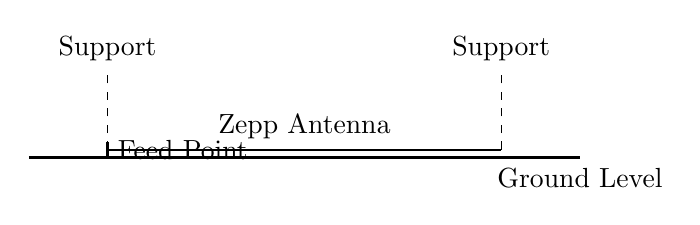
\begin{tikzpicture}
    % Draw the antenna
    \draw[thick] (0,0) -- (5,0) node[midway, above] {Zepp Antenna};
    \draw[thick] (0,-0.1) -- (0,0.1) node[midway, right] {Feed Point};
    
    % Draw support structures
    \draw[dashed] (0,0) -- (0,1) node[above] {Support};
    \draw[dashed] (5,0) -- (5,1) node[above] {Support};
    
    % Add ground
    \draw[thick] (-1,-0.1) -- (6,-0.1) node[below] {Ground Level};
\end{tikzpicture}
\end{center}

This diagram shows the basic layout of a Zepp antenna with a feed point at one end and supports at both ends.
